\subsection{Overview}

\begin{frame}{Project Overview}

\begin{itemize}
\item \framac may handle several ASTs in the same session
\item a project groups together one AST with all the global data attached to it
\item examples of such data are
  \begin{itemize}
  \item the AST itself
  \item kernel tables like those of kernel functions and annotations
  \item command line options
  \item results of analyzers
  \end{itemize}
\item such data are called states
\item by default, each operation are applied on the current project
\end{itemize}

\end{frame}

%%%%%%%%%%%%%%%%%%%%%%%%%%%%%%%%%%%%%%%%%%%%%%%%%%%%%%%%%%%%%%%%%%%%%%%%%%%%%%%

\begin{frame}{Client/Server View}
  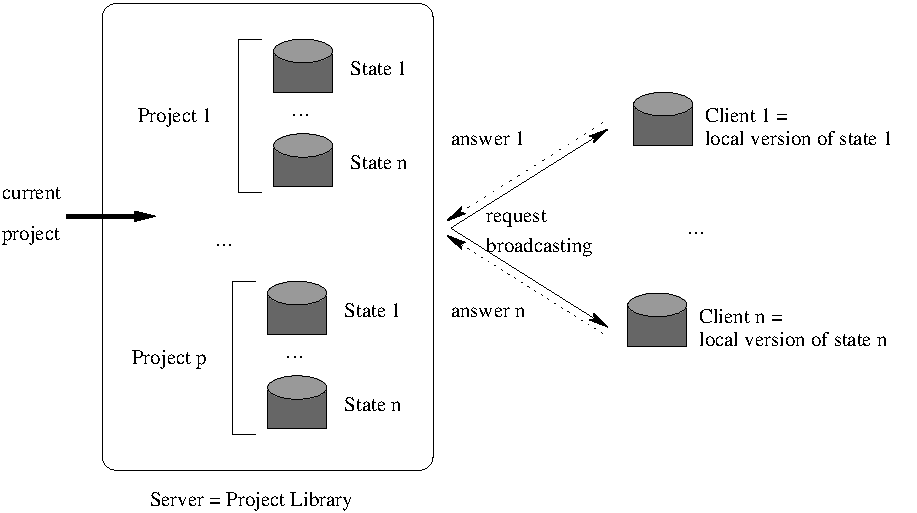
\includegraphics[scale=0.68]{mecanisme.pdf}

  \begin{itemize}
  \item delayed synchronization between client $i$ and server' state $i$
    of the current project    
  \end{itemize}
\end{frame}

%%%%%%%%%%%%%%%%%%%%%%%%%%%%%%%%%%%%%%%%%%%%%%%%%%%%%%%%%%%%%%%%%%%%%%%%%%%%%%%

\subsection{State}

\begin{frame}{State}
  \framesubtitle{Overview}

\begin{itemize}
\item each time you create a global data, ask yourself: "is this data part of a
  project or common to all projects?"
\item most often, it is really part of a project
\item in such cases, you have to create a \emph{projectified state} (otherwise
  use standard \ocaml datastructures like references or hashtables)
\end{itemize}

\end{frame}

%%%%%%%%%%%%%%%%%%%%%%%%%%%%%%%%%%%%%%%%%%%%%%%%%%%%%%%%%%%%%%%%%%%%%%%%%%%%%%%

\begin{frame}[fragile]{State}
  \framesubtitle{Registration Overview}

\begin{itemize}
\item module \lstinline+State_builder+
\item a state is a module created through functor application
\item low-level functor \lstinline+State_builder.Register+
\item several high-level functors
  \begin{itemize}
  \item \lstinline+State_builder.Ref+
  \item \lstinline+State_builder.Option_ref+
  \item \lstinline+State_builder.Set_ref+
  \item \lstinline+State_builder.Hashtbl+
  \item \lstinline+State_builder.Queue+
  \item \lstinline+State_builder.Counter+
  \item ...
  \end{itemize}
\item much simpler to use them (prefer a reference to a record than a mutable
  record, even if less efficient...)
\end{itemize}

\end{frame}

%%%%%%%%%%%%%%%%%%%%%%%%%%%%%%%%%%%%%%%%%%%%%%%%%%%%%%%%%%%%%%%%%%%%%%%%%%%%%%%

\begin{frame}[fragile]{State}
  \framesubtitle{Registration in Practice}

\begin{ocamlcode}
module My_bool_ref = 
  False_ref(struct
    let name = "My_plugin.My_bool_ref"
    let dependencies = []
    let kind = `Correctness
  end)
\end{ocamlcode}

\end{frame}

%%%%%%%%%%%%%%%%%%%%%%%%%%%%%%%%%%%%%%%%%%%%%%%%%%%%%%%%%%%%%%%%%%%%%%%%%%%%%%%

\begin{frame}[fragile]{State}
  \framesubtitle{Registration in Practice (2)}

\begin{ocamlcode}
type callstack = 
  (Cil_types.stmt * Kernel_function.t) list

module My_callstack =
  State_builder.Ref
    (Datatype.List
      (Cil_datatype.Stmt)(Kernel_function))
    (struct 
      let name = "My_plugin.My_callstack"
      let dependencies = 
        [ Ast.self; Kernel_function.self ]
      let kind = `Correctness
      let default () = []
     end)
\end{ocamlcode}

\end{frame}

%%%%%%%%%%%%%%%%%%%%%%%%%%%%%%%%%%%%%%%%%%%%%%%%%%%%%%%%%%%%%%%%%%%%%%%%%%%%%%%

\begin{frame}[fragile]{State}
  \framesubtitle{Registration in Practice (3)}

\begin{ocamlcode}
module My_hashtbl =
  State_builder.Hashtbl
    (Cil_datatype.Stmt.Hashtbl)
    (Datatype.String)
    (struct 
      let name = "My_plugin.My_hashtbl"
      let dependencies = [ Ast.self ]
      let kind = `Correctness
      let size = 17
     end)
\end{ocamlcode}

\end{frame}

%%%%%%%%%%%%%%%%%%%%%%%%%%%%%%%%%%%%%%%%%%%%%%%%%%%%%%%%%%%%%%%%%%%%%%%%%%%%%%%

\begin{frame}[fragile]{State}
  \framesubtitle{Use}

\begin{ocamlcode}
open Cil_types
let _ = object (self)
  inherit Visitor.frama_c_inplace
  method vinst = function
    | Call(_ret_lval, 
           { enode = Lval(Var v, NoOffset) }, 
           _args, 
           _loc) ->
      My_callstack.set
        ((Option.get self#current_stmt,
          Globals.Functions.get v)
        :: (My_callstack.get ()));
      Cil.SkipChildren
    | _ -> Cil.SkipChildren	
end
\end{ocamlcode}

\end{frame}

%%%%%%%%%%%%%%%%%%%%%%%%%%%%%%%%%%%%%%%%%%%%%%%%%%%%%%%%%%%%%%%%%%%%%%%%%%%%%%%

\subsection{Project Operations}

\begin{frame}[fragile]{Project Operations}

  \begin{itemize}
  \item \lstinline+Project.current+
  \item \lstinline+Project.create+, \lstinline+Project.remove+
  \item \lstinline+Project.copy+
  \item \lstinline+Project.save+, \lstinline+Project.load+
  \item  \lstinline+Project.set_current+, \lstinline+Project.on+
\begin{ocamlcode}
let main () =
  let p =
    Sparecode.Register.get
      ~select_annot:false
      ~select_slice_pragma:false
   in
   Project.on p Eva.Analysis.compute ()
\end{ocamlcode}
  \end{itemize}

\end{frame}

%%%%%%%%%%%%%%%%%%%%%%%%%%%%%%%%%%%%%%%%%%%%%%%%%%%%%%%%%%%%%%%%%%%%%%%%%%%%%%%

\subsection{State Selection}

\begin{frame}{State Selection}
  \framesubtitle{Overview}
  \begin{itemize}
  \item project operations may be applied only on some states
  \item such a set of states is called a \emph{state selection}
  \item a way to improve efficiency
  \item a way to easily implement some operations over states (like clearing)
  \item must preserve \framac's global consistency
  \item that is the \emph{raison d'\^etre} of \emph{state dependencies} which
    allows to easily specify consistent selections
  \end{itemize}
\end{frame}

%%%%%%%%%%%%%%%%%%%%%%%%%%%%%%%%%%%%%%%%%%%%%%%%%%%%%%%%%%%%%%%%%%%%%%%%%%%%%%%

\begin{frame}[fragile]{State Selection}
  \framesubtitle{Example}
  
  \begin{ocamlcode}
(* clear value analysis' results
   and all its depending state
   in the current project *)
let selection =
  State_selection.Dynamic.with_dependencies 
    !Db.Value.self
in
Project.clear ~selection ()
  \end{ocamlcode}

\end{frame}

%%%%%%%%%%%%%%%%%%%%%%%%%%%%%%%%%%%%%%%%%%%%%%%%%%%%%%%%%%%%%%%%%%%%%%%%%%%%%%%

\subsection{Marshaling}

\begin{frame}{Marshaling}
\end{frame}
